\apendice{Especificación de Requisitos}

\section{Introducción}
La herramienta \textit{Olivia Finder} tiene como objetivo principal proporcionar
una gestión eficiente de paquetes y dependencias de diferentes repositorios, como
\textit{PyPI}, \textit{npm}, \textit{CRAN} y \textit{Bioconductor}. Para lograr esto,
hemos identificado una serie de requisitos funcionales que guiarán el diseño y la
implementación del sistema.

El primer requisito funcional, \texttt{RF-1}, se centra en el almacenamiento eficiente
y el acceso rápido a la información de paquetes y dependencias. Es fundamental que el
sistema pueda almacenar esta información de manera eficiente para evitar demoras
significativas en la recuperación de datos. Además, el acceso rápido a la información
permitirá un rendimiento óptimo del sistema.

La extensibilidad y flexibilidad de la estructura de datos es abordada por el
requisito \texttt{RF-2}. Dado que los repositorios y las relaciones de dependencia
pueden evolucionar con el tiempo, es esencial que la estructura de datos utilizada sea
adaptable y pueda ser modificada o ampliada sin dificultades. Esto garantizará que el
sistema pueda adaptarse a futuras modificaciones en los repositorios y en las necesidades
de gestión de dependencias.

El requisito \texttt{RF-3} se enfoca en la representación específica de paquetes mediante
una estructura de datos adecuada. Cada paquete debe tener una representación clara y
precisa, que incluya los atributos relevantes para dicho paquete. Esto facilitará la
gestión y el análisis de los paquetes y sus dependencias dentro del sistema.

El requisito \texttt{RF-4} se refiere a la representación y exportación genérica de la
red de dependencias en diferentes formatos. Es importante que la red de dependencias
pueda ser representada en formatos genéricos de grafo dirigido, así como en otros formatos
como diccionarios, listas o dataframes. Esta versatilidad en la representación y exportación
permitirá un uso más amplio de la red de dependencias en diferentes herramientas y análisis.

La reconstrucción de las estructuras de datos a través de la persistencia es abordada por
el requisito \texttt{RF-5}. El sistema debe ser capaz de reconstruir las estructuras de
datos utilizadas para almacenar la información de paquetes y dependencias a partir de una
forma persistente, como archivos o bases de datos. Esto garantizará la integridad de
los datos y facilitará la continuidad del trabajo en caso de interrupciones o reinicios del sistema.

El requisito \texttt{RF-6} se centra en el almacenamiento de datos adicionales sobre la
relación de dependencia entre los paquetes. Además de las dependencias directas, es
importante capturar información adicional, como la versión concreta utilizada, para
permitir un análisis más completo y detallado de las relaciones de dependencia.

El sistema debe ser capaz de obtener datos de manera eficiente desde múltiples fuentes, este
es el requisito \texttt{RF-7}. Esto incluye la capacidad de leer archivos CSV, acceder a
APIs de terceros o realizar web scraping para obtener la información necesaria de los
repositorios. Esta funcionalidad flexible garantizará una amplia variedad de opciones para
obtener los datos requeridos por el sistema.

El requisito \texttt{RF-8} se refiere a la obtención de dependencias transitivas de forma dinámica durante la ejecución
del sistema. Esto implica obtener tanto las dependencias directas como las dependencias
indirectas de un paquete en tiempo real. Esta funcionalidad permitirá un análisis más completo
de las relaciones de dependencia y facilitará la toma de decisiones basada en dichas dependencias.

Por último, el requisito \texttt{RF-9} se centra en el manejo de excepciones. El sistema
debe implementar un mecanismo para capturar y manejar adecuadamente situaciones excepcionales
que puedan surgir durante su ejecución. Esto incluye la generación de mensajes de error
claros y la posibilidad de gestionar los errores de manera adecuada para minimizar su
impacto en la funcionalidad general del sistema.

\section{Catálogo de requisitos funcionales}

\begin{itemize}
	\item \textbf{RF-1: Almacenamiento eficiente y acceso rápido a la información de paquetes y dependencias}.

	      El sistema debe ser capaz de almacenar la información de manera eficiente y permitir un acceso rápido a los paquetes y sus dependencias, evitando demoras significativas.

	\item \textbf{RF-2: Extensibilidad y flexibilidad de la estructura de datos para futuras modificaciones}.

	      La estructura de datos utilizada para representar los paquetes y dependencias debe ser flexible y adaptable, de modo que pueda ser modificada o ampliada en el futuro sin dificultades.

	\item \textbf{RF-3: Representación específica de paquetes mediante una estructura de datos adecuada}.

	      Cada paquete debe tener una representación clara y precisa mediante una estructura de datos que contenga los atributos relevantes para dicho paquete.

	\item \textbf{RF-4: Representación y exportación genérica de la red de dependencias en diferentes formatos}.

	      La red de dependencias debe poder ser representada y exportada en formatos genéricos de grafo dirigido, así como en otros formatos como diccionario, listas o dataframes, permitiendo una mayor versatilidad en su uso.

	\item \textbf{RF-5: Reconstrucción de estructuras de datos a través de la persistencia}.

	      El sistema debe ser capaz de reconstruir las estructuras de datos utilizadas para almacenar la información de paquetes y dependencias a partir de una forma persistente, como archivos o bases de datos.

	\item \textbf{RF-6: Almacenamiento de datos adicionales sobre la relación de dependencia}.

	      Se requiere la capacidad de almacenar información adicional sobre la relación de dependencia entre los paquetes, como la versión concreta utilizada, para capturar detalles específicos y permitir un análisis más completo.

	\item \textbf{RF-7: Obtención eficiente de datos desde múltiples fuentes}.

	      El sistema debe ser capaz de obtener datos de manera eficiente desde diversas fuentes, como archivos CSV, APIs de terceros o mediante web scraping, permitiendo una amplia variedad de opciones para obtener la información necesaria.

	\item \textbf{RF-8: Obtención de dependencias transitivas dinámicamente en tiempo de ejecución}.

	      Se debe permitir la obtención de dependencias transitivas de un paquete de forma dinámica durante la ejecución del sistema, lo que implica obtener las dependencias directas e indirectas de un paquete en tiempo real.

	\item \textbf{RF-9: Manejo de excepciones para capturar y manejar situaciones excepcionales}.

	      El sistema debe implementar un mecanismo para capturar y manejar adecuadamente las situaciones excepcionales que puedan ocurrir durante su ejecución, proporcionando información clara sobre los fallos y permitiendo una gestión adecuada de los errores.
\end{itemize}

\section{Catálogo de requisitos no funcionales}

\begin{itemize}
	\item \textbf{RNF-1: Usabilidad.}

	      Es necesario que la biblioteca proporcione a los usuarios una manera sencilla y
	      bien documentada de obtener redes de dependencia. Esto implica aplicar principios, mecanismos y sistemas de organización
	      de código ampliamente utilizados en el lenguaje, de modo que la interfaz de la biblioteca se adapte a la experiencia,
	      las expectativas y los modelos mentales de los usuarios.

	\item \textbf{RNF-2: Rendimiento.}

	      Las funciones de la biblioteca deben tener la capacidad de ejecutarse de manera eficiente
	      en equipos domésticos, incluso al trabajar con redes grandes. Se considerará como un caso de prueba el rendimiento del software
	      al operar con la red de paquetes npm (\textit{Node.js}). El objetivo principal de este requisito es permitir un uso ágil e interactivo,
	      facilitando la exploración y la investigación, y también asegurando que la biblioteca pueda ser aprovechada por una amplia gama
	      de usuarios, que incluyen gestores de repositorios centralizados, desarrolladores de software y desarrolladores de herramientas
	      de calidad continua.

	\item \textbf{RNF-3: Mantenimiento y extensibilidad.}

	      El diseño de la biblioteca debe estar orientado a facilitar el mantenimiento
	      correctivo y evolutivo. Esto implica adoptar una estructura y una arquitectura que permitan realizar modificaciones y expansiones
	      de manera eficiente, sin ocasionar interrupciones significativas en el funcionamiento del software.

	\item \textbf{RNF-4: Documentación.}

	      Es fundamental que la solución esté adecuadamente documentada. Con el propósito de facilitar
	      su divulgación, toda la documentación será redactada en inglés. Esto incluye la inclusión de documentación en el código mediante
	      el uso de docstrings, siguiendo estándares comunes en este aspecto, así como la provisión de ejemplos prácticos que ilustren el
	      uso de las funciones de la biblioteca.

	\item \textbf{RNF-5: Soporte.}

	      La biblioteca debe ser compatible con versiones superiores a \textit{Python3.8}. Esto garantiza que
	      la biblioteca pueda ser utilizada en entornos actuales y futuros basados en Python, asegurando así su viabilidad y utilidad a
	      largo plazo.
\end{itemize}

\section{Casos de uso}

Los casos de uso son una técnica para capturar los requisitos funcionales de un sistema. Se trata de una
descripción de las acciones que realiza un usuario y las respuestas del sistema ante dichas acciones.
Los casos de uso se representan mediante diagramas de casos de uso, que muestran las relaciones entre los distintos actores y casos de uso del sistema.

A continuacion presentamos los casos de uso del sistema, que se han agrupado en dos grupos: casos de uso de la biblioteca y casos de uso de los notebooks.

\subsection{Casos de uso de la biblioteca}

\begin{figure}[ht!]
	\centering
	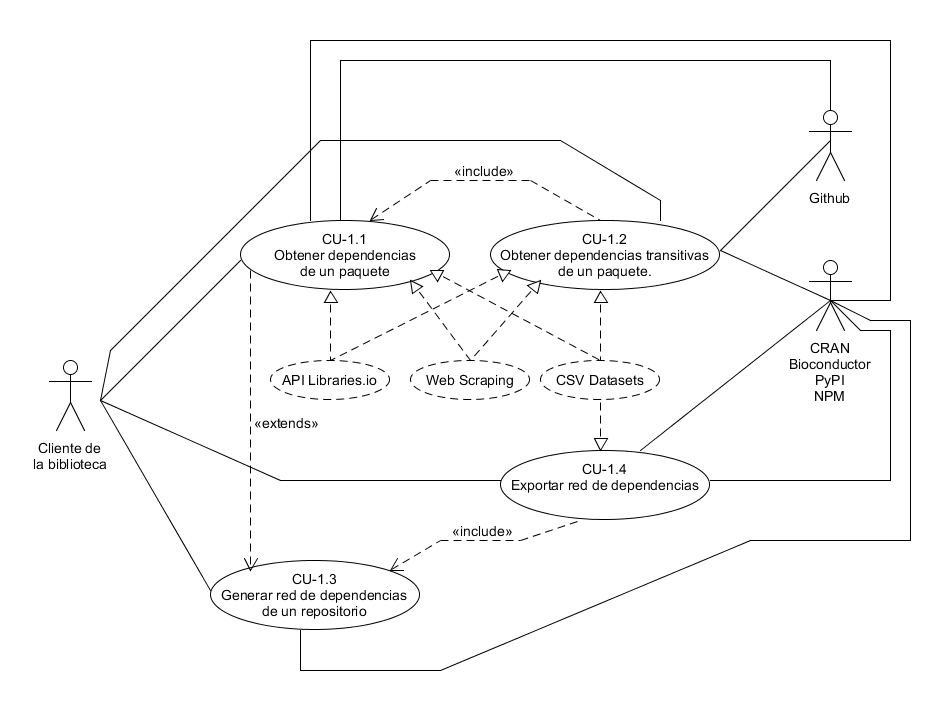
\includegraphics[width=1\textwidth]{img/anexos/CU_of.png}
	\caption{Diagrama de casos de uso de la biblioteca Olivia Finder.}
	\label{fig:casos_de_uso}
\end{figure}

Los casos de uso de la biblioteca se muestran representados en un diagrama de casos de uso en la figura \ref{fig:casos_de_uso}.
Los actores que interactúan con el sistema son el usuario y los repositorios de paquetes.

\textbf{CU-1.1: Obtener dependencias de un paquete.}

\begin{table}[p]
	\centering
	\begin{tabularx}{\linewidth}{ p{0.21\columnwidth} p{0.71\columnwidth} }
		\toprule
		\textbf{CU-1.1}               & \textbf{Obtención de las dependencias de un paquete}                              \\
		\toprule
		\textbf{Versión}              & 1.0                                                                              \\
		\textbf{Autor}                & Daniel Alonso                                                                    \\
		\textbf{Requisitos asociados} & RF-1, RF-2, RF-3, RF-6, RF-7, RF-8, RF-9                                         \\
		\textbf{Descripción}          & Obtener las dependencias de un paquete de las redes
		PyPI, npm, CRAN, Bioconductor y GitHub.                                                                          \\
		\textbf{Precondición}         & Las fuentes de datos usadas para obtener las dependencias
		deben de estar accesibles.                                                                                       \\
		\textbf{Acciones}             &
		\begin{enumerate}
			\def\labelenumi{\arabic{enumi}.}
			\tightlist
			\item Identificar el paquete del cual se desean obtener las dependencias.
			\item Realizar una búsqueda en la fuente de datos para obtener las dependencias del paquete.
		\end{enumerate}                      \\
		\textbf{Postcondición}        & Se obtienen las dependencias del paquete en formato diccionario.                 \\
		\textbf{Excepciones}          & Si el paquete no existe en alguna de las redes, se obtiene un diccionario vacío. \\
		\textbf{Importancia}          & Media                                                                            \\
		\bottomrule
	\end{tabularx}
	\caption{CU-1 Dependencias de un paquete.}
	\label{tab:cu1}
\end{table}

El caso de uso \texttt{CU-1.1} \ref{tab:cu1} se centra en la obtención de las dependencias de un paquete específico. Permite
identificar el paquete deseado y realizar una búsqueda en las fuentes de datos correspondientes, como PyPI,
npm, CRAN, Bioconductor y GitHub. Al finalizar, se obtiene un diccionario que contiene las dependencias del
paquete, lo que resulta útil para comprender las relaciones y requisitos del software.



\textbf{CU-1.2: Obtener dependencias transitivas de un paquete.}

\begin{table}[p]
	\centering
	\begin{tabularx}{\linewidth}{ p{0.21\columnwidth} p{0.71\columnwidth} }
		\toprule
		\textbf{CU-1.2}               & \textbf{Obtención de las dependencias transitivas de un paquete}                                       \\
		\toprule
		\textbf{Versión}              & 1.0                                                                                                    \\
		\textbf{Autor}                & Daniel Alonso                                                                                          \\
		\textbf{Requisitos asociados} & RF-1, RF-3, RF-7, RF-8, RF-9                                                                           \\
		\textbf{Descripción}          & Obtener las dependencias transitivas de un paquete, utilizando una profundidad de búsqueda específica. \\
		\textbf{Precondición}         & Las dependencias directas del paquete están disponibles y las fuentes de datos son accesibles.         \\
		\textbf{Acciones}             &
		\begin{enumerate}
			\def\labelenumi{\arabic{enumi}.}
			\tightlist
			\item Identificar el paquete del cual se desean obtener las dependencias transitivas.
			\item Establecer la profundidad de búsqueda deseada.
			\item Recorrer recursivamente las dependencias directas del paquete hasta alcanzar la profundidad de búsqueda establecida.
			\item Registrar todas las dependencias transitivas encontradas durante el recorrido.
		\end{enumerate}              \\
		\textbf{Postcondición}        & Se obtienen las dependencias transitivas del paquete hasta la profundidad de búsqueda especificada.    \\
		\textbf{Excepciones}          & Si el paquete no existe en las redes de paquetes, se añade como un diccionario vacio.                  \\
		\textbf{Importancia}          & Media                                                                                                  \\
		\bottomrule
	\end{tabularx}
	\caption{CU-2 Dependencias transitivas de un paquete.}
	\label{tab:cu2}
\end{table}

Por otro lado, el caso de uso \texttt{CU-1.2} \ref{tab:cu2} se enfoca en la obtención de las dependencias transitivas de un paquete.
Permite establecer una profundidad de búsqueda y recorrer de manera recursiva las dependencias directas del
paquete hasta alcanzar dicha profundidad. Durante este proceso, se registran todas las dependencias transitivas
encontradas. Esto es beneficioso para comprender el impacto y alcance de un paquete, así como las dependencias
indirectas que pueden influir en su funcionamiento.


\textbf{CU-1.3: Generar red de dependencias de un repositorio.}

\begin{table}[p]
	\centering
	\begin{tabularx}{\linewidth}{ p{0.21\columnwidth} p{0.71\columnwidth} }
		\toprule
		\textbf{CU-1.3}               & \textbf{Generación de la red de dependencias de un repositorio}                                                          \\
		\toprule
		\textbf{Versión}              & 1.0                                                                                                                      \\
		\textbf{Autor}                & Daniel Alonso                                                                                                            \\
		\textbf{Requisitos asociados} & RF-3, RF-5, RF-6, RF-7, RF-9                                                                                             \\
		\textbf{Descripción}          & Generar la red de dependencias de paqutes para un repositorio.                                                           \\
		\textbf{Precondición}         & Los repositorios PyPI, npm, CRAN y Bioconductor están accesibles via Web o disponemos de otra fuente de datos soportada. \\
		\textbf{Acciones}             &
		\begin{enumerate}
			\def\labelenumi{\arabic{enumi}.}
			\tightlist
			\item Obtener la lista de paquetes disponibles en el repositorio.
			\item Para cada paquete, obtener sus dependencias directas.
			\item Construir la red de dependencias, donde los paquetes son los nodos y las relaciones de dependencia son los enlaces.
		\end{enumerate}                                 \\
		\textbf{Postcondición}        & Se genera la red de dependencias que muestra las relaciones entre los paquetes en el repositorio.                        \\
		\textbf{Excepciones}          & Si no es posible acceder a alguno de los repositorios, se obtiene una excepcion.                                         \\
		\textbf{Importancia}          & Alta                                                                                                                     \\
		\bottomrule
	\end{tabularx}
	\caption{CU-3 Red de dependencias.}
	\label{tab:cu3}
\end{table}

El caso de uso \texttt{CU-1.3} \ref{tab:cu3} se refiere a la generación de la red de dependencias de un repositorio. Este caso de uso
implica obtener la lista de paquetes disponibles en el repositorio y, para cada paquete, identificar sus
dependencias directas. Posteriormente, se construye una red de dependencias donde los paquetes son los nodos
y las relaciones de dependencia son los enlaces. Esta representación visual de las dependencias proporciona
una visión clara y estructurada de cómo los paquetes interactúan entre sí en el repositorio.



\textbf{CU-1.4: Exportar red de dependencias.}

\begin{table}[p]
	\centering
	\begin{tabularx}{\linewidth}{ p{0.21\columnwidth} p{0.71\columnwidth} }
		\toprule
		\textbf{CU-1.4}               & \textbf{Exportación de la red de dependencias}                                                                                                   \\
		\toprule
		\textbf{Versión}              & 1.0                                                                                                                                              \\
		\textbf{Autor}                & Daniel Alonso                                                                                                                                    \\
		\textbf{Requisitos asociados} & RF-3, RF-4, RF-6                                                                                                                                 \\
		\textbf{Descripción}          & Almacenar la red de dependencias para su uso posterior por otras herramientas o análisis, asegurando la compatibilidad con la biblioteca OLIVIA. \\
		\textbf{Precondición}         & Se ha generado la red de dependencias correctamente.                                                                                             \\
		\textbf{Acciones}             &
		\begin{enumerate}
			\def\labelenumi{\arabic{enumi}.}
			\tightlist
			\item Exportar la red de dependencias en un formato compatible con la biblioteca OLIVIA.
			\item Guardar el archivo de exportación en una ubicación adecuada para su uso posterior.
		\end{enumerate}                                                                                          \\
		\textbf{Postcondición}        & La red de dependencias se almacena en un formato compatible con la biblioteca OLIVIA para su posterior utilización.                              \\
		\textbf{Excepciones}          &                                                                                                                                                  \\
		\textbf{Importancia}          & Alta                                                                                                                                             \\
		\bottomrule
	\end{tabularx}
	\caption{CU-4 Exportación de la red.}
	\label{tab:cu4}
\end{table}

El caso de uso \texttt{CU-1.4} \ref{tab:cu4} se encarga de la exportación de la red de dependencias generada. Permite
almacenar la red en un formato compatible con la biblioteca \textit{OLIVIA}, asegurando su posterior utilización por
otras herramientas o análisis. Al exportar la red, se garantiza la preservación de la información sobre las
dependencias, lo que facilita su intercambio y colaboración con otros sistemas o investigadores interesados
en el análisis de paquetes y sus interconexiones.

\newpage

\subsection{Casos de uso de un cliente de la biblioteca \textit{Olivia Finder}}

\begin{figure}[ht!]
	\centering
	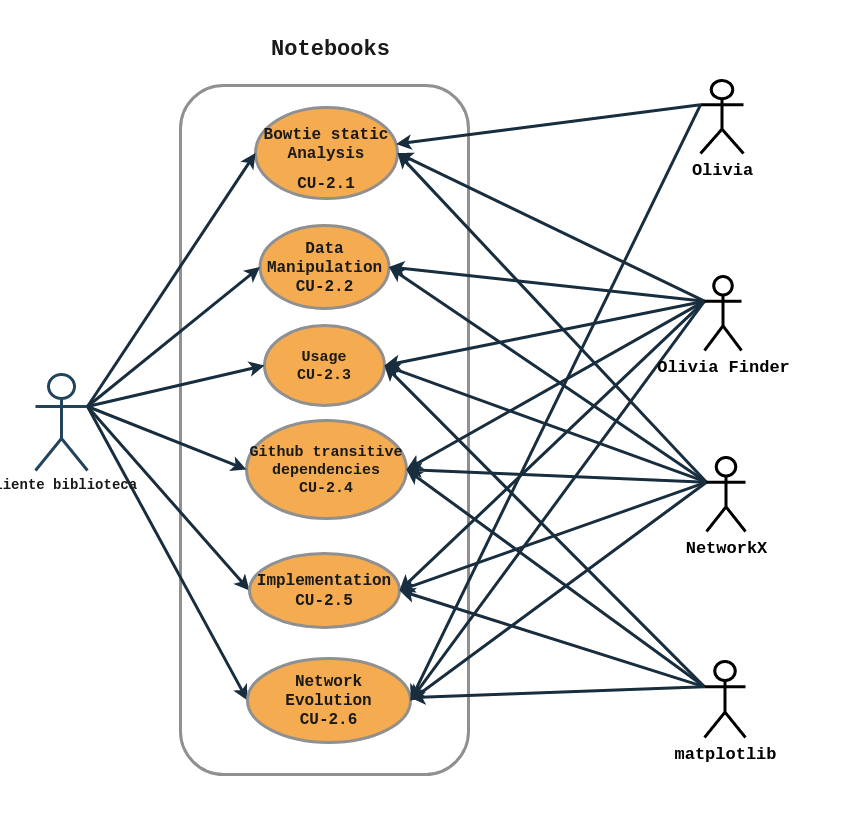
\includegraphics[width=1\textwidth]{img/anexos/CU_notebooks.png}
	\caption{Diagrama de casos de uso de los clientes de la biblioteca.}
	\label{fig:casos_de_uso_notebooks}
\end{figure}

Los casos de uso de los clientes de la biblioteca se muestran en la figura \ref{fig:casos_de_uso_notebooks}.


\textbf{CU-2.1: Análisis estático de Bow-tie.}

\begin{table}[p]
	\centering
	\begin{tabularx}{\linewidth}{ p{0.21\columnwidth} p{0.71\columnwidth} }
		\toprule
		\textbf{CU-2.1}               & \textbf{Análisis estático de Bow-tie}                                         \\
		\toprule
		\textbf{Versión}              & 1.0                                                                           \\
		\textbf{Autor}                & Daniel Alonso                                                                 \\
		\textbf{Requisitos asociados} & RF-1, RF-2, RF-3, RF-7, RF-8, RNF-1, RNF-2, RNF-4                             \\
		\textbf{Descripción}          & Realizar un análisis comparativo de las métricas
		obtenidas para conjuntos de datos utilizando una estructura de Bowtie y las métricas
		de vulnerabilidad en OLIVIA.                                                                                  \\
		\textbf{Precondición}         & Se han obtenido los conjuntos de datos y se han definido
		las métricas de vulnerabilidad en OLIVIA.                                                                     \\
		\textbf{Acciones}             &
		\begin{enumerate}
			\def\labelenumi{\arabic{enumi}.}
			\tightlist
			\item Aplicar la estructura de Bowtie a los conjuntos de datos.
			\item Calcular las métricas de vulnerabilidad definidas en OLIVIA para cada conjunto de datos.
			\item Realizar una comparativa de las métricas obtenidas.
		\end{enumerate}                 \\
		\textbf{Postcondición}        & Se obtiene un análisis comparativo de las métricas obtenidas
		para los conjuntos de datos utilizando una estructura de Bowtie y las métricas de
		vulnerabilidad en OLIVIA.                                                                                     \\
		\textbf{Excepciones}          & No se pueden obtener los conjuntos de datos o las métricas de vulnerabilidad. \\
		\textbf{Importancia}          & Alta                                                                          \\
		\bottomrule
	\end{tabularx}
	\caption{CU-2.1 Análisis estático de Bowtie.}
	\label{tab:cu2.1}
\end{table}

El \textit{Notebook} \textit{Bow-tie static analysis}\footnote{Idea sacada del artículo:
	"many directed networks show a structure where most nodes belong to a WCC that can be
	partitioned into three main subsets: the largest SCC, the set of nodes that can reach the
	SCC, i.e. the IN set, and the set of nodes that can be reached from the SCC, i.e. the OUT
	set, which is usually represented in the form of a bow-tie diagram~\cite{Broder2000309}} lleva a cabo un análisis comparativo de las
métricas obtenidas para conjuntos de datos utilizando una estructura de Bow-tie\cite{enwiki:1148363387} y
las métricas de vulnerabilidad definidas en \textit{OLIVIA}. \ref{tab:cu2.1}



\textbf{CU-2.2: Manipulación de datos.}

El caso de uso de \textit{Manipulación de datos} muestra como realizar la obtenición de datos utilizando \textit{Olivia Finder}.
En concreto se muestra como se construye un objeto \texttt{PackageManager} usando las distintas fuentes de datos implementadas y cómo se pueden combinar, con el fin de obtener las dependencias
de los paquetes y entender la forma en que se presentan estos datos. \ref{tab:cu2.2}

\begin{table}[p]
	\centering
	\begin{tabularx}{\linewidth}{ p{0.21\columnwidth} p{0.71\columnwidth} }
		\toprule
		\textbf{CU-2.2}               & \textbf{Manipulación de datos}                                                      \\
		\toprule
		\textbf{Versión}              & 1.0                                                                                 \\
		\textbf{Autor}                & Daniel Alonso                                                                       \\
		\textbf{Requisitos asociados} & RF-1, RF-2, RF-3, RF-4, RF-5, RF-7, RF-9, RNF-1, RNF-2, RNF-4                       \\
		\textbf{Descripción}          & Realizar los pasos necesarios para manipular los datos
		utilizando \textit{Olivia Finder}, con el objetivo de obtener las dependencias de los
		paquetes y comprender cómo se presentan los datos.                                                                  \\
		\textbf{Precondición}         & \textit{Olivia Finder} ha sido configurado correctamente y los datos
		de los paquetes están disponibles.                                                                                  \\
		\textbf{Acciones}             & \begin{enumerate}
			                                \item Utilizar \textit{Olivia Finder} para obtener las dependencias de los paquetes.
			                                \item Analizar la forma en que se presentan los datos obtenidos.
		                                \end{enumerate} \\
		\textbf{Postcondición}        & Se comprende la forma en que se presentan los datos de las
		dependencias de los paquetes, lo que permite su posterior manipulación y análisis.                                  \\
		\textbf{Excepciones}          & No se pueden obtener las dependencias de los paquetes
		utilizando \textit{Olivia Finder}.                                                                                  \\
		\textbf{Importancia}          & Alta                                                                                \\
		\bottomrule
	\end{tabularx}
	\caption{CU-2.2 Manipulación de datos.}
	\label{tab:cu2.2}
\end{table}

\textbf{CU-2.3: Selección de estrategias de extracción de datos.}

El caso de uso \textit{Selección de estrategias de extracción de datos} presenta un procedimiento para generar un conjunto de datos
(lista de enlaces) con la red de dependencias deseada, y proporciona directrices sobre cómo
utilizarlo para realizar un análisis estático. \ref{tab:cu2.3}

\begin{table}[p]
	\centering
	\begin{tabularx}{\linewidth}{ p{0.21\columnwidth} p{0.71\columnwidth} }
		\toprule
		\textbf{CU-2.3}               & \textbf{Selección de estrategias de extracción de datos}                                                   \\
		\toprule
		\textbf{Versión}              & 1.0                                                                                                        \\
		\textbf{Autor}                & Daniel Alonso                                                                                              \\
		\textbf{Requisitos asociados} & RF-1, RF-2, RF-3, RF-7, RF-9, RNF-1, RNF-2, RNF-4                                                          \\
		\textbf{Descripción}          & Generar un conjunto de datos (lista de enlaces) con la red de dependencias
		deseada y proporcionar directrices sobre cómo utilizarlo para realizar un análisis estático.                                               \\
		\textbf{Precondición}         & Los datos de la red de dependencias y las directrices de análisis están
		disponibles.                                                                                                                               \\
		\textbf{Acciones}             & \begin{enumerate}
			                                \item Generar un conjunto de datos (lista de enlaces) que represente la red de dependencias deseada.
			                                \item Proporcionar directrices sobre cómo utilizar el conjunto de datos para realizar un análisis estático.
		                                \end{enumerate} \\
		\textbf{Postcondición}        & Se dispone de un conjunto de datos que representa la red de dependencias
		deseada y se conocen las directrices para realizar un análisis estático utilizando dicho
		conjunto.                                                                                                                                  \\
		\textbf{Excepciones}          & No se pueden generar los datos de la red de dependencias o las
		directrices de análisis están ausentes o incorrectas.                                                                                      \\
		\textbf{Importancia}          & Alta                                                                                                       \\
		\bottomrule
	\end{tabularx}
	\caption{CU-2.3 Uso.}
	\label{tab:cu2.3}
\end{table}

\textbf{CU-2.4: Dependencias transitivas de un repositorio de GitHub.}

El caso de uso de \textit{Dependencias transitivas de un repositorio de GitHub} está diseñado para obtener las dependencias transitivas de un repositorio
en \textit{GitHub}. Se basa en una exploración exhaustiva de las dependencias de un paquete,
alcanzando la profundidad deseada en el árbol de dependencias. \ref{tab:cu2.4}

\begin{table}[p]
	\centering
	\begin{tabularx}{\linewidth}{ p{0.21\columnwidth} p{0.71\columnwidth} }
		\toprule
		\textbf{CU-2.4}               & \textbf{Dependencias transitivas de un repositorio de GitHub}                                                                                                              \\
		\toprule
		\textbf{Versión}              & 1.0                                                                                                                                                                        \\
		\textbf{Autor}                & Daniel Alonso                                                                                                                                                              \\
		\textbf{Requisitos asociados} & RF-1, RF-2, RF-3, RF-4, RF-5, RF-7, RF-9, RNF-1, RNF-2, RNF-4                                                                                                              \\
		\textbf{Descripción}          & Obtener las dependencias transitivas de un repositorio en GitHub mediante una exploración exhaustiva de las dependencias de un paquete, alcanzando la profundidad deseada. \\
		\textbf{Precondición}         & Se ha especificado el repositorio objetivo y se ha definido la profundidad deseada para la exploración de dependencias.                                                    \\
		\textbf{Acciones}             & \begin{enumerate}
			                                \item Identificar el repositorio objetivo en GitHub.
			                                \item Realizar una exploración exhaustiva de las dependencias del paquete, alcanzando la profundidad deseada en el árbol de dependencias.
			                                \item Registrar las dependencias transitivas obtenidas.
		                                \end{enumerate}                                   \\
		\textbf{Postcondición}        & Se obtienen las dependencias transitivas del repositorio objetivo, registradas y listas para su análisis posterior.                                                        \\
		\textbf{Excepciones}          & No se puede acceder al repositorio en GitHub o no se encuentran las dependencias del paquete en el repositorio.                                                            \\
		\textbf{Importancia}          & Alta                                                                                                                                                                       \\
		\bottomrule
	\end{tabularx}
	\caption{CU-2.4 Dependencias transitivas de GitHub.}
	\label{tab:cu2.4}
\end{table}


\textbf{CU-2.5: Detalles de implementación (Para programadores).}

Este caso de uso, pese a ser muy genérico proporciona una guía detallada para desarrolladores sobre la implementación
de la herramienta, mostrando las funcionalidades de los distintos módulos. Ofrece una visión en
profundidad de la biblioteca y sus componentes. Esta pensado introducir de una forma descriptiva el funcionamiento de la biblioteca
a un nivel mas bajo y ser de ayuda para el programador que decida hacer reimplementaciones de la biblioteca. \ref{tab:cu2.5}

\begin{table}[p]
	\centering
	\begin{tabularx}{\linewidth}{ p{0.21\columnwidth} p{0.71\columnwidth} }
		\toprule
		\textbf{CU-2.5}               & \textbf{Implementación}                                                                                                                              \\
		\toprule
		\textbf{Versión}              & 1.0                                                                                                                                                  \\
		\textbf{Autor}                & Daniel Alonso                                                                                                                                        \\
		\textbf{Requisitos asociados} & RF-1, RF-2, RF-3, RF-4, RF-5, RF-6, RF-7, RF-8, RF-9, RNF-1, RNF-2, RNF-3, RNF-4, RNF-5                                                              \\
		\textbf{Descripción}          & Proporcionar una guía detallada para el desarrollador sobre la implementación de la herramienta, mostrando las funcionalidades de los módulos.       \\
		\textbf{Precondición}         & Se ha realizado la implementación de la herramienta y se dispone de los módulos correspondientes.                                                    \\
		\textbf{Acciones}             & \begin{enumerate}
			                                \item Describir las funcionalidades de los módulos de la herramienta.
			                                \item Explicar el uso adecuado de cada módulo y sus componentes.
			                                \item Proporcionar ejemplos de código para ilustrar la implementación.
		                                \end{enumerate}                                                                                \\
		\textbf{Postcondición}        & El desarrollador obtiene una visión en profundidad de la biblioteca y sus componentes, lo que facilita la implementación y el uso de la herramienta. \\
		\textbf{Excepciones}          & Problemas en la herramienta o faltan los módulos correspondientes.                                                                                   \\
		\textbf{Importancia}          & Alta                                                                                                                                                 \\
		\bottomrule
	\end{tabularx}
	\caption{CU-2.5 Implementación.}
	\label{tab:cu2.5}
\end{table}

\textbf{CU-2.6: Evolución de la red.}

El caso de uso de \textit{Evolución de la red} presentan un análisis evolutivo de los repositorios
desde una perspectiva experimental. Se realiza un análisis gráfico
básico de cómo ha variado el repositorio a lo largo del tiempo, utilizando los datos
de \textit{libraries.io}\cite{jeremy_katz_2020_3626071} del año 2020 y los datos obtenidos mediante \textit{Olivia Finder} en el 2023. \ref{tab:cu2.6}


\begin{table}[p]
	\centering
	\begin{tabularx}{\linewidth}{ p{0.21\columnwidth} p{0.71\columnwidth} }
		\toprule
		\textbf{CU-2.6}               & \textbf{Evolución de la red}                                                                                                                                                              \\
		\toprule
		\textbf{Versión}              & 1.0                                                                                                                                                                                       \\
		\textbf{Autor}                & Daniel Alonso                                                                                                                                                                             \\
		\textbf{Requisitos asociados} & RF-1, RF-4, RF-7, RF-9, RNF-1, RNF-2, RNF-4, RNF-5                                                                                                                                        \\
		\textbf{Descripción}          & Realizar un análisis evolutivo de los repositorios desde una perspectiva experimental, proporcionando un análisis gráfico básico de cómo ha variado el repositorio a lo largo del tiempo. \\
		\textbf{Precondición}         & Se disponen de los datos de \textit{libraries.io} del año 2020 y de los datos obtenidos mediante \textit{Olivia Finder}.                                                                  \\
		\textbf{Acciones}             & \begin{enumerate}
			                                \item Utilizar los datos de \textit{libraries.io} y de \textit{Olivia Finder} para analizar la evolución de los repositorios.
			                                \item Generar gráficos que ilustren cómo ha variado el repositorio a lo largo del tiempo.
			                                \item Realizar un análisis comparativo de los resultados obtenidos.
		                                \end{enumerate}                                                              \\
		\textbf{Postcondición}        & Se obtiene un análisis evolutivo de los repositorios, que proporciona una visión básica de cómo ha variado el repositorio a lo largo del tiempo.                                          \\
		\textbf{Excepciones}          & No se disponen de los datos de \textit{libraries.io} del año 2020 o de los datos obtenidos mediante \textit{Olivia Finder}.                                                               \\
		\textbf{Importancia}          & Alta                                                                                                                                                                                      \\
		\bottomrule
	\end{tabularx}
	\caption{CU-2.6 Evolución de la red.}
	\label{tab:cu2.6}
\end{table}


\section{Objetivos generales}

Los objetivos generales de este Trabajo de Fin de Grado se centran en la obtención de conjuntos de
datos de los repositorios de software \textit{CRAN}, \textit{Bioconductor}, \textit{PyPI} y \textit{npm},
con el propósito de generar redes de dependencias de paquetes.

Estos objetivos se concretan en el desarrollo de la biblioteca \textit{Olivia Finder}, una herramienta
que permite la adquisición de datos, manipulación y exportación en formatos compatibles con la
biblioteca \textit{OLIVIA} y otras bibliotecas de análisis de redes, como \textit{NetworkX}.

Con el fin de obtener una visión más completa de la red de dependencias de los repositorios
seleccionados, se incluirán análisis evolutivos que reflejen los estados y cambios en dichos repositorios.
Estos análisis proporcionarán información sobre el tamaño, distribución de grado y otras métricas de
centralidad relevantes para los paquetes presentes en los repositorios.

Además, se lleva a cabo un esfuerzo en la descripción del funcionamiento de la biblioteca, con el objetivo 
de asegurar su mantenimiento y continuidad en el desarrollo, mejoras y ampliación de funcionalidades. Se 
documentan \textit{funcionalidades}, \textit{estructuras de datos} y \textit{flujos de trabajo}. Se destaca 
la importancia de mantener una arquitectura modular, lo que facilita la incorporación 
de nuevas características sin afectar la estabilidad general del sistema. Asimismo, se establecen estándares 
de codificación y buenas prácticas para asegurar la legibilidad del código y favorecer la colaboración entre 
desarrolladores. La documentación resultante actúa como un recurso valioso para el equipo de desarrollo y 
la comunidad de usuarios para mantener con vida la biblioteca.

% \section{Catálogo de requisitos}

% \section{Especificación de requisitos}





